\chapter{Nombre Comparaisons}
Les tableau suivant représente les nombre de comparaison des algorithmes de tri selon la configuration du tableau.
\section{Tableau trie en bon ordre}
\small
\begin{center}
\resizebox{15cm}{!}{
\begin{tabular}{| c | c | c | c | c |  }
    \hline
     N &   10000 & 50000 & 10^5 & 5*10^5  \\
    \hline
    Tri par selection & 49995000 &	1249975000 &	4999950000 & 124999750000	 \\
    \hline
    Tri par insertion & 9999 & 49999 & 99999 & 499999\\
    \hline
    Tri par fusion & 1336310&	7844810&	16689460&	94757320	\\
    \hline
    Tri a bulle & 16588 &
56783 &
107007 &
508329  \\
    \hline
    Tri tas & 244460 & 1455438 & 3112517 & 17837785 		 \\
    \hline
    Tri rapide (Début) & 25005000 & 625025000 & 12500050000 & 62500250000\\
    \hline
    Tri rapide (Fin) & 49995001 & 1249975001& 4999950001 & 124999750001  \\
    \hline
    Tri rapide (Millieu) & 180011 & 1003409 & 2106802 & 11927156	 \\
    \hline
\end{tabular}}
\end{center}
\normalsize
La figure suivante représente l’évolution des nombres de comparaisons selon la taille du tableau 100000 
\begin{figure}[H]
    \centering
        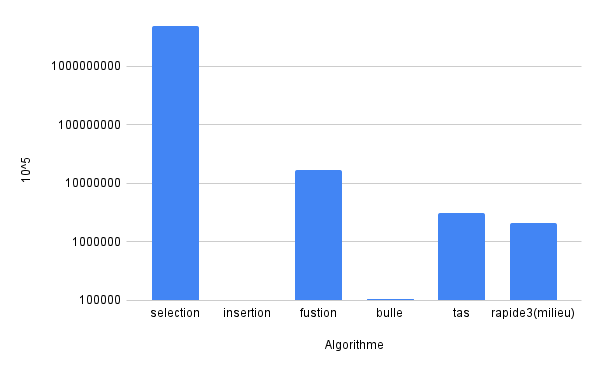
\includegraphics[scale=0.7]{ressources/comordre.png}
        \caption{nombre des comparaisons selon l'algorithme}
    \label{fig:temps_exec_dico_theo}
\end{figure} 
\par
Depuis le graphe, on observe que le nombre de comparaison dans la meilleur cas des algorithmes fusion , selection , tas et rapide est tres eleves par rapport aux algorithmes insertion et bulle.  
\par
\begin{figure}[H]
    \centering
        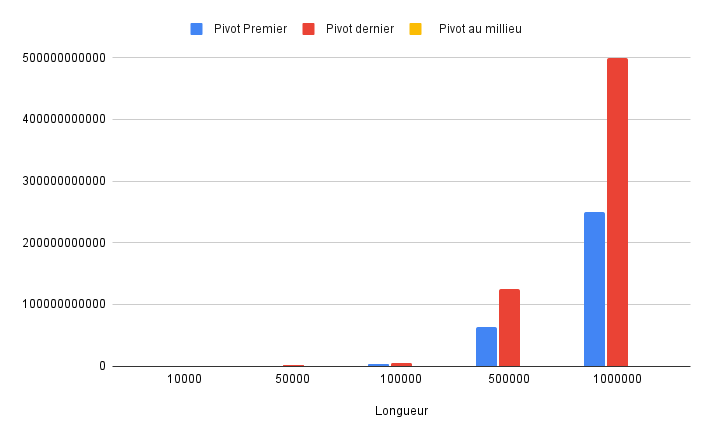
\includegraphics[scale=0.7]{ressources/nb_triee.png}
        \caption{Nombre des comparaisons effectuées par les  algorithmes de Tri Rapide selon la taille du tableau}
    \label{fig:temps_exec_dico_theo}
\end{figure} 
\par
\section{Tableau trie en ordre inverse}
\small
\begin{center}
\resizebox{15cm}{!}{
\begin{tabular}{| c | c | c | c | c |  }
    \hline
     N &   10000 & 50000 & 10^5 & 5*10^5  \\
    \hline
    Tri par selection & 49995000 &	1249975000	 & 4999950000 &	124999750000	 \\
    \hline
    Tri par insertion & 49995000 & 1249975000 & 4999950000 & 12499750000  \\
    \hline
    Tri par fusion & 1336310&	7844810&	16689460&	94757320	\\
    \hline
    Tri a bulle & 50001245 &
1250026893 &
5001098891 &
5001098891 	 \\
    \hline
    Tri tas &  226682 & 1366047 & 2926640 & 16977997   \\
    \hline
    Tri rapide (Début) & 50005000 & 1250025000 & 5000050000 & 125000250000  \\
    \hline
    Tri rapide (Fin) & 50005000 & 1250025000& 5000050000 & /  \\
    \hline
    Tri rapide (Millieu) & 143169 & 848331 & 1796637 & 9786465  \\
    \hline
\end{tabular}}
\end{center}
\normalsize
La figure suivante représente l’évolution du nombre de comparaisons selon l'algorithme utilisé avec une taille du tableau 100000 
\begin{figure}[H]
    \centering
        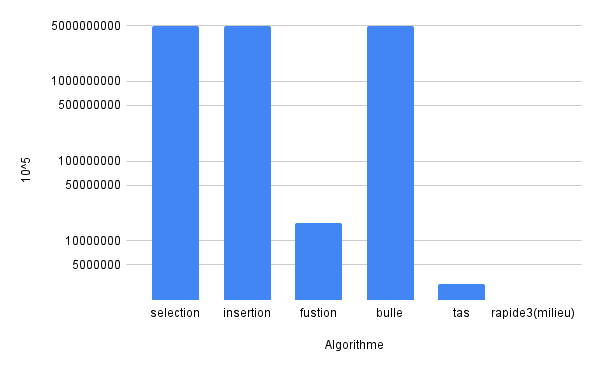
\includegraphics[scale=0.7]{ressources/cominverse.png}
        \caption{nombre des comparaisons selon l'algorithme}
    \label{fig:temps_exec_dico_theo}
\end{figure} 
\par
Depuis le graphe, on observe que le nombre de comparaison des algorithmes selection ,insertion et bulle est tres eleves par rapport aux autres algorithmes fusion , tas , et le tri rapide donnent des meilleurs resultats. 
\par
\begin{figure}[H]
    \centering
        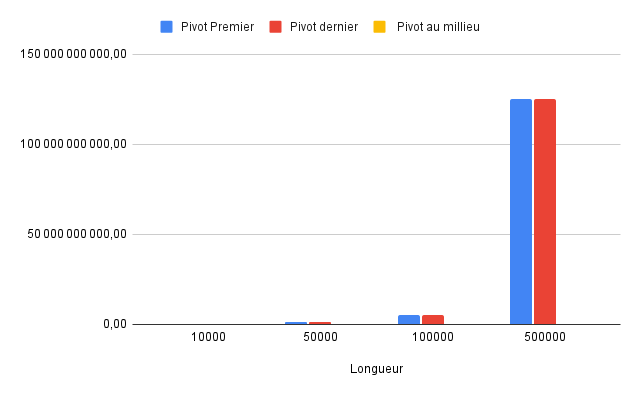
\includegraphics[scale=0.7]{ressources/nb_inv.png}
        \caption{Nombre des comparaisons effectuées par les  algorithmes de Tri Rapide selon la taille du tableau}
    \label{fig:temps_exec_dico_theo}
\end{figure} 
\par
\section{Tableau trie aleatoirement}
\small
\begin{center}
\resizebox{15cm}{!}{
\begin{tabular}{| c | c | c | c | c |  }
    \hline
     N &   10000 & 50000 & 10^5 & 5*10^5  \\
    \hline
    Tri par selection & 49995000 & 	1249975000	& 4999950000	& 124999750000	 \\
    \hline
    Tri par insertion & 25234406 &  623931087 & 2492077689 & 62470481149 \\
    \hline
    Tri par fusion & 1336310&	7844810&	16689460&	94757320		\\
    \hline
    Tri a bulle & 50002183 &
1250010338 &
5003278417 & //  \\
    \hline
    Tri tas &   235334 & 1409925 & 3019611 & 17397152   \\
    \hline
     Tri rapide (Début) & 161015 & 978870 & 12056258 & 11881598  \\
    \hline
    Tri rapide (Fin) & 168562 & 993500 & 2141419 & 12216452 	 \\
    \hline
    Tri rapide (Millieu) & 262726 & 1474652 & 3184007 & 18730250	 \\
    \hline
    
\end{tabular}}
\end{center}
\normalsize
La figure suivante représente l’évolution du nombre de comparaisons selon l'algorithme utilisé avec une taille du tableau 100000
\begin{figure}[H]
    \centering
        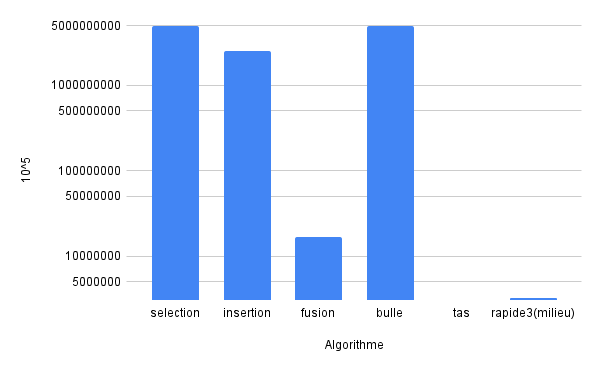
\includegraphics[scale=0.7]{ressources/comaleatoire.png}
        \caption{nombre des comparaisons selon l'algorithme}
    \label{fig:temps_exec_dico_theo}
\end{figure} 
\par
Depuis le graphe, on observe que le nombre de comparaison des algorithmes selection ,insertion et bulle est très elevés par rapport aux autres algorithmes fusion , rapide et tas avec meilleur complexite. 
\normalsize

\section{Conclusion}
depuis les graphes , on observe que le nombre des comparaisons represénte quasiment la complexité de l'algorithme ainsi qu'ils existent des algorithmes de comparaisons qui ne sont pas couteux en nombres de comparaisons effectuées et ils sont privilégiés dans la pratique dans le cas où la comparaison est dispendieuse.

